\chapter{Dialogbeispiele}
\label{chapter-dialogbeispiel}
Der folgende Abschnitt präsentiert das in der vorliegenden Arbeit realisierte
System anhand eines beispielhaften Nutzungsszenarios. Das Szenario startet mit
Mila, einer Erstsemester-Studentin im Studiengang Medieninformatik. Mila belegt
im ersten Semester das Modul \textit{\ac{emi}}. Das Einführungsmodul umfasst
eine Gruppenarbeit, in der eine Idee zum Thema \textit{VR/AR} entwickelt werden
soll. Am Ende des Semesters soll das Projekt bei den \textit{Media Moments} in
der \textit{\ac{emi} Award App} \cite{UniversitatzuLubeck2021} ausgestellt werden.
Milas Projektgruppe hat sich entschieden, eine AR-Anwendung für Erze und Metalle
zu gestalten, bei der diese mithilfe einer App eingescannt werden
können und ihre entsprechenden Eigenschaften angezeigt werden. Um das Projekt in
der \textit{\ac{emi} Award App} präsentieren zu können, will die Gruppe ein
Werbevideo für die App aufnehmen.

In einem Videoworkshop von Georg Fink, \ac{wimi} am \ac{imis}, erfahren
Mila und ihre Gruppenmitglieder:innen, dass über die Ausleih-App
\textit{Snipe-IT Companion} unter anderem Videoequipment an Studierende
verliehen wird.

Mila ruft die Ausleih-App unter der URL \textit{https://snipe-it-companion.de/} auf und meldet sich
mit ihren Daten an. Daraufhin wird sie zu einem bisher leeren \textit{Dashboard} weitergeleitet und
aufgefordert, nach benötigtem Material zu suchen. Da Mila sich nicht sicher ist, welche Kamera sie
benötigt, schaut sich Mila unter dem Menü in den Kategorien um und findet schnell die Kategorie
\enquote{Kameras} (\ref{fig:login}). Nachdem sie auf die Seite der Unterkategorien weitergeleitet
wurde, entscheidet sich Mila dafür, eine \textit{GoPro} auszuleihen, weil sie so auch Erze und
Metalle unter Wasser aufnehmen kann. Dazu klickt Mila auf \enquote{Hinzufügen} (\ref{fig:suchen}).
\begin{figure}[p]
    \centering
    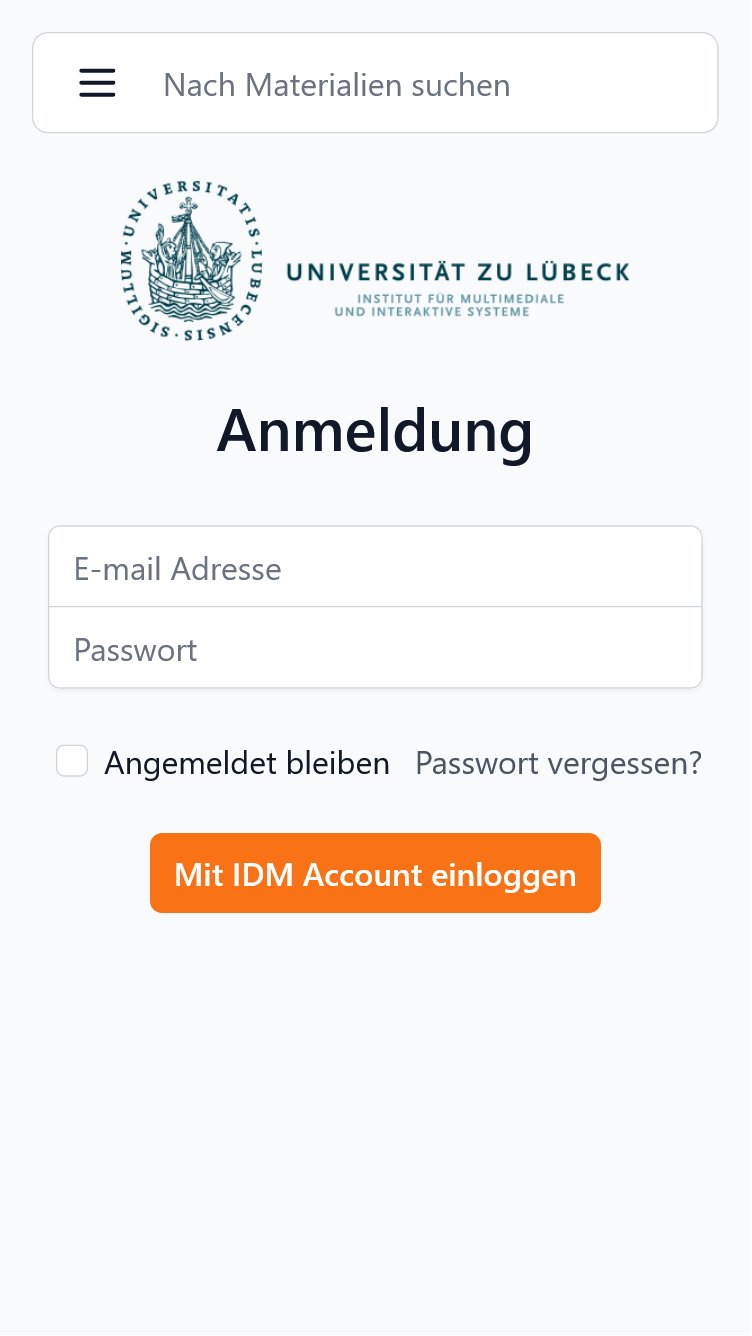
\includegraphics[scale=0.17]{Bilder/Dialgobeispiel/Login.png}\hspace{1em}
    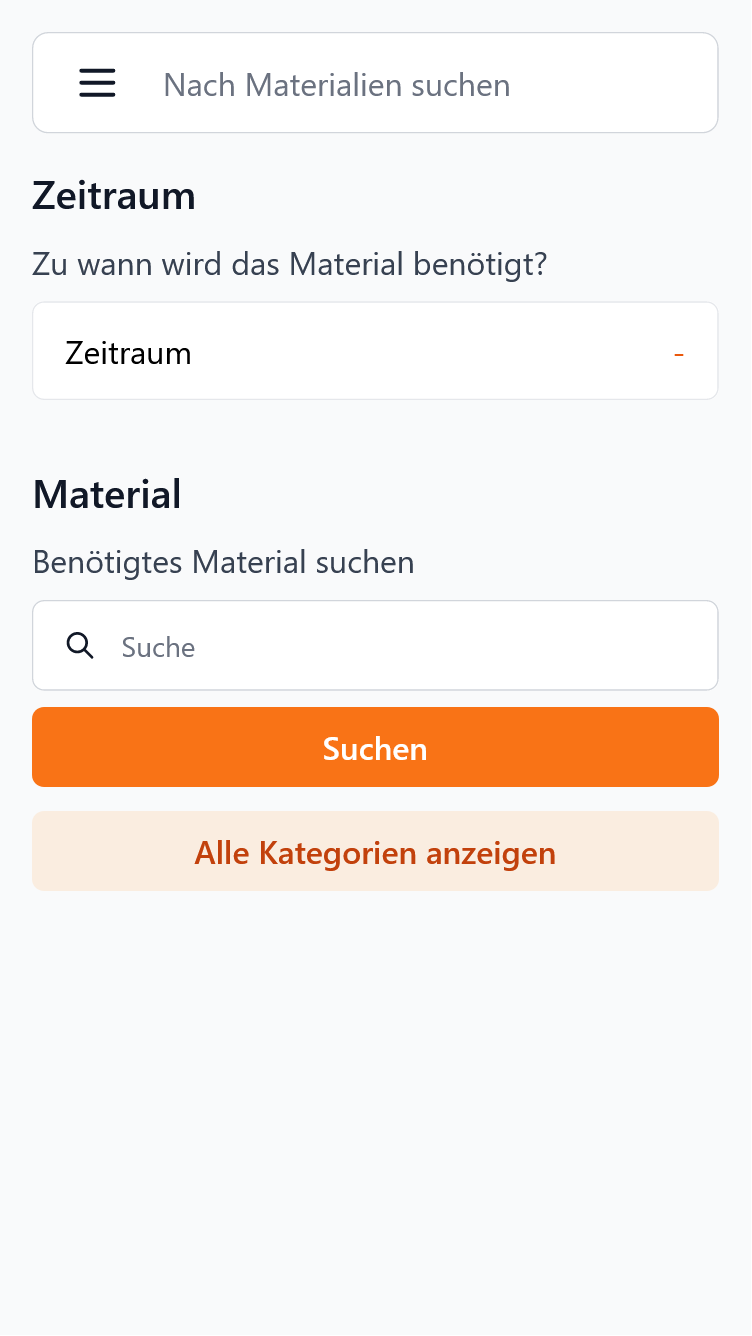
\includegraphics[scale=0.17]{Bilder/Dialgobeispiel/Suiche2.png} \hspace{1em}
    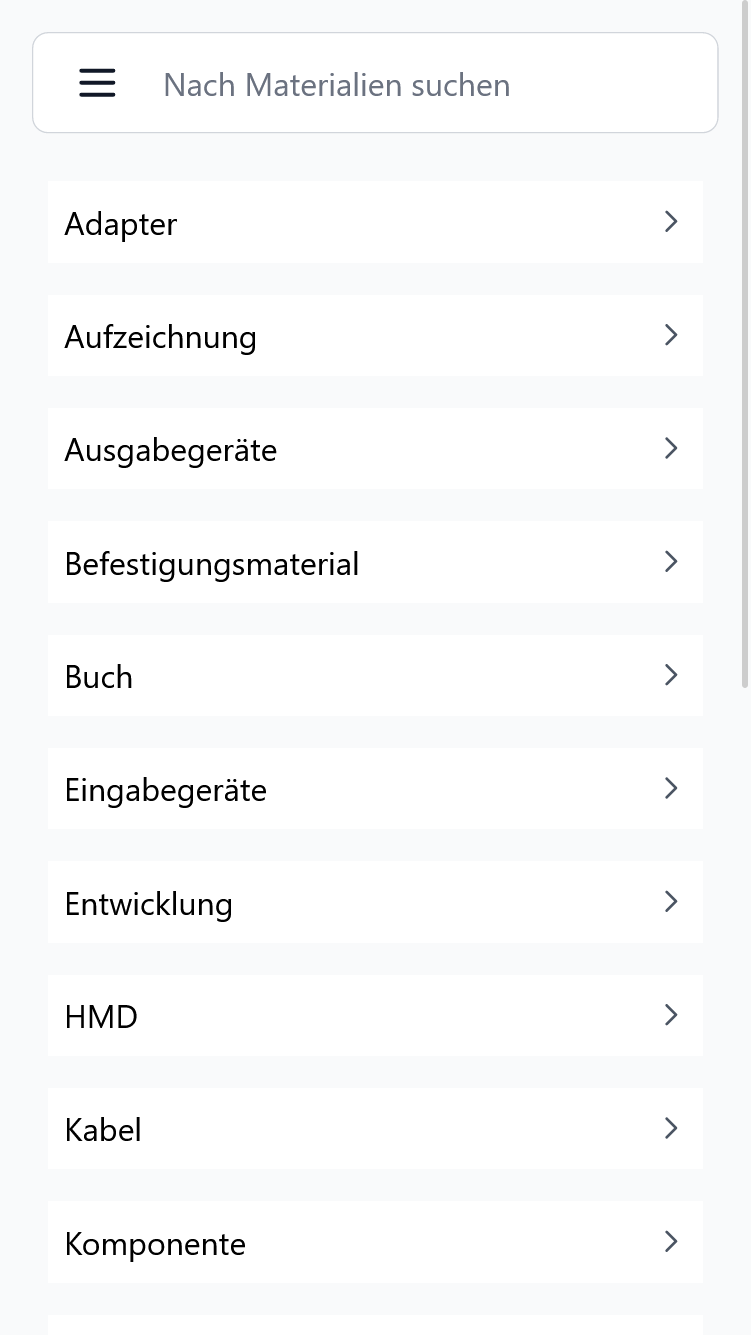
\includegraphics[scale=0.17]{Bilder/Dialgobeispiel/Kategorien.png}
    \caption{Dialogbeispiel 1: Einloggen, Suche, Kategorien}\label{fig:login}
\end{figure}
\begin{figure}[p]
    \centering
    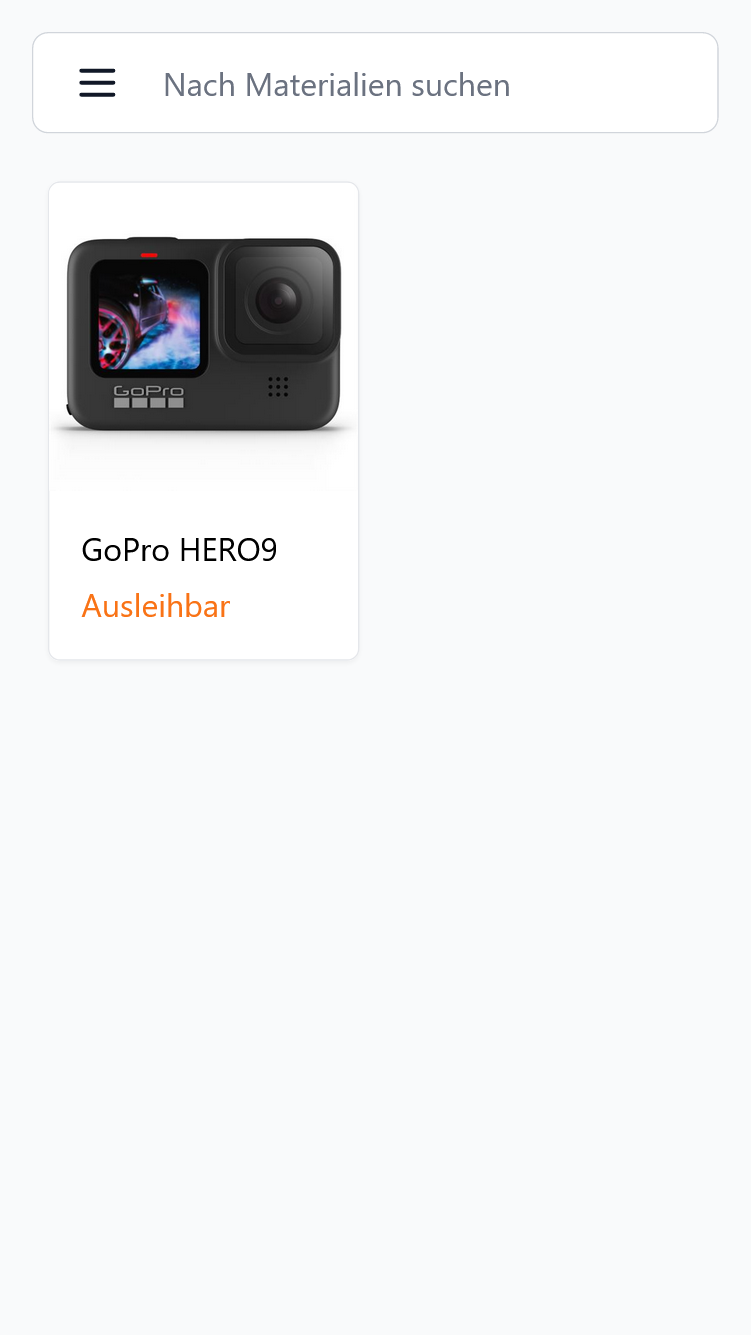
\includegraphics[scale=0.17]{Bilder/Dialgobeispiel/Suche.png}\hspace{1em}
    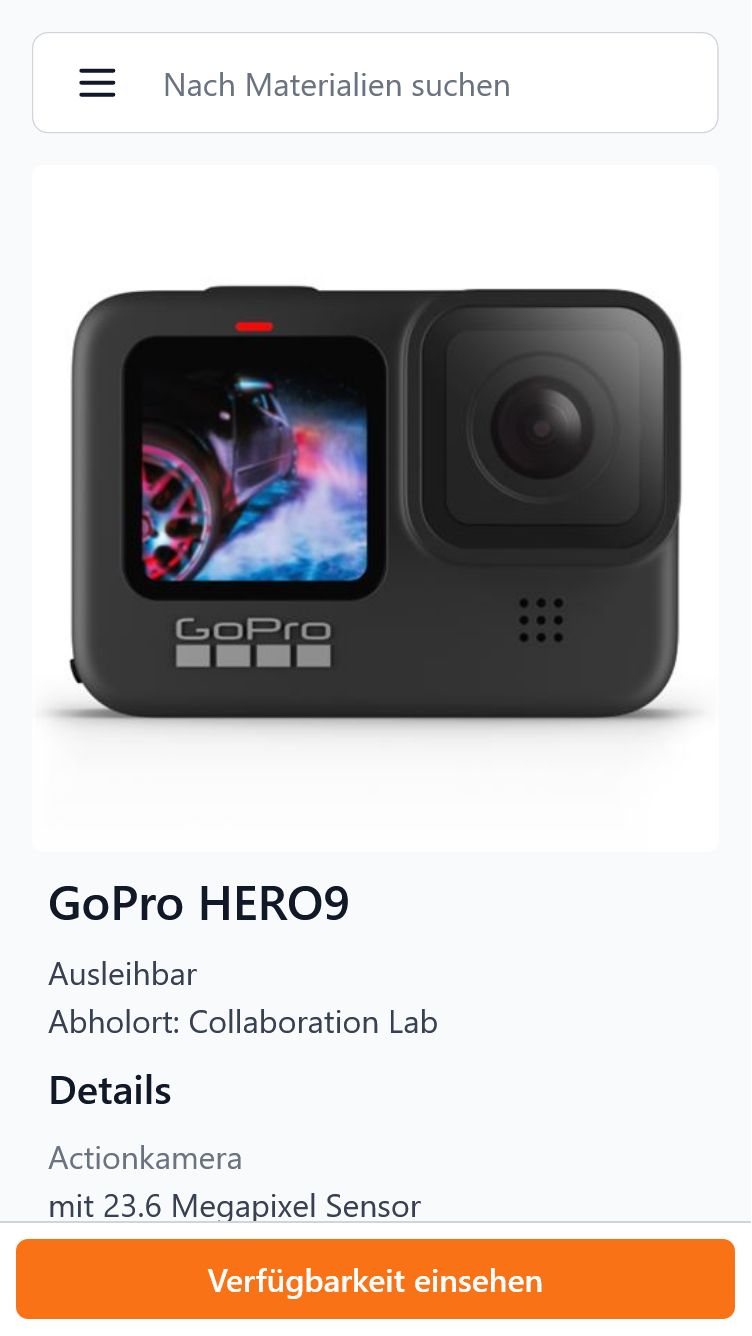
\includegraphics[scale=0.17]{Bilder/Dialgobeispiel/Details 1.png} \hspace{1em}
    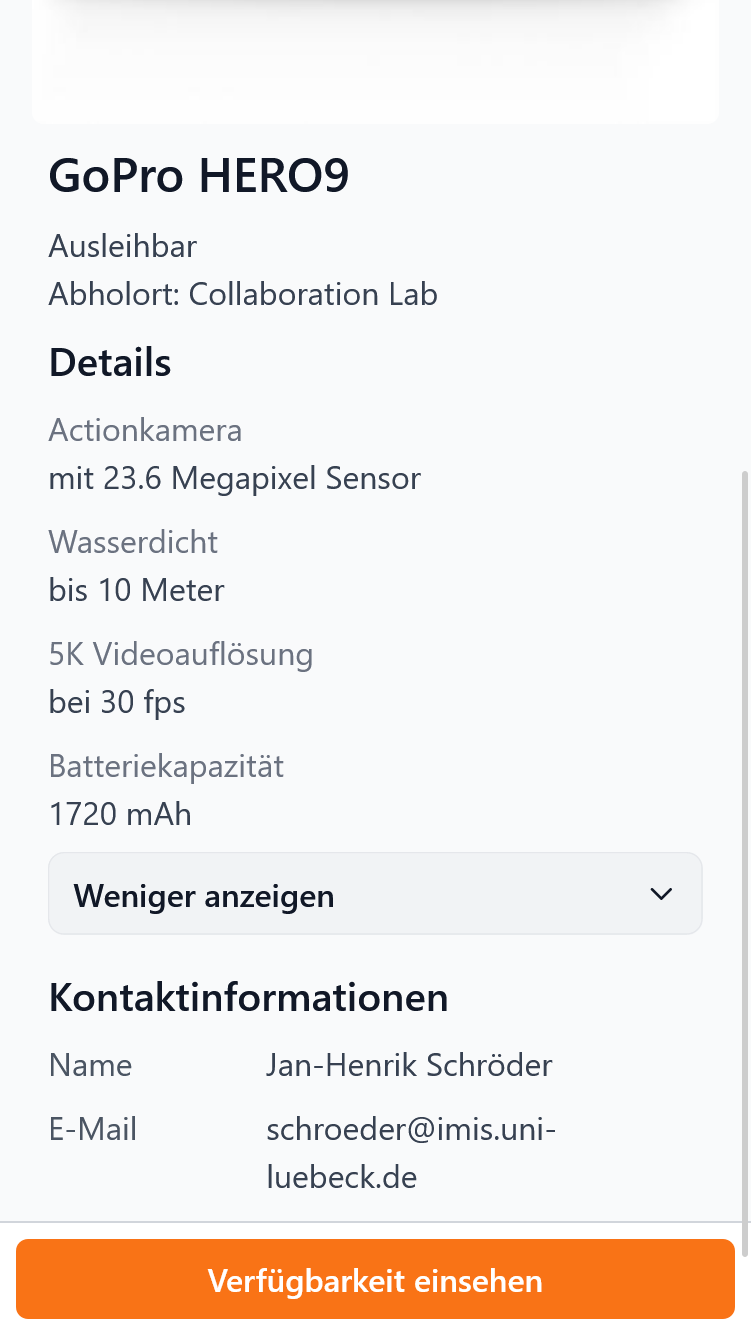
\includegraphics[scale=0.17]{Bilder/Dialgobeispiel/Details 2.png}
    \caption{Dialogbeispiel 2: Suchergebnisse (Kacheln), Detailansicht}\label{fig:suchen}
\end{figure}

\newpage
Nun wird sie dazu aufgefordert, einen Ausleihzeitraum anzugeben. Milas Gruppe hat entschieden, dass
sie das Material von kommenden Montag bis Mittwoch benötigen. Da Mila von 8:00 Uhr bis 10:00 Uhr eine Vorlesung
hat, gibt sie jeweils 10:30 Uhr als Abholzeit und Rückgabezeit an. Um die Reservierung abschließen zu
können, klickt Mila auf \enquote{Reservieren} (\ref{fig:datum}). Mila überprüft in der
Zusammenfassung, ob ihre Angaben stimmen und stellt fest, dass die Rückgabezeit am Mittwoch doch
nicht mehr in ihren Kalender passt. Daher ändert sie die Uhrzeit auf 12:30 Uhr und bestätigt
abschließend ihre Reservierung (\ref{fig:geandert}).

\begin{figure}[p]
    \centering
    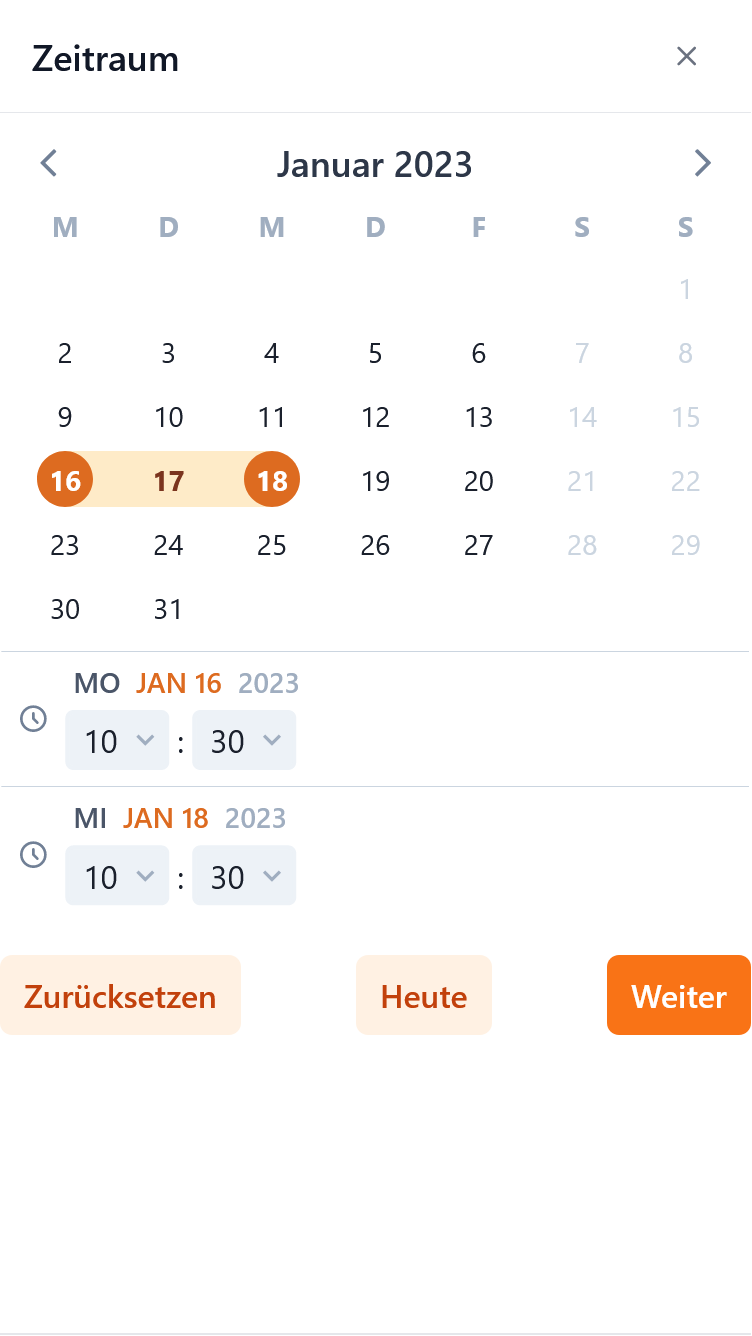
\includegraphics[scale=0.17]{Bilder/Dialgobeispiel/Datum eingeben.png}\hspace{1em}
    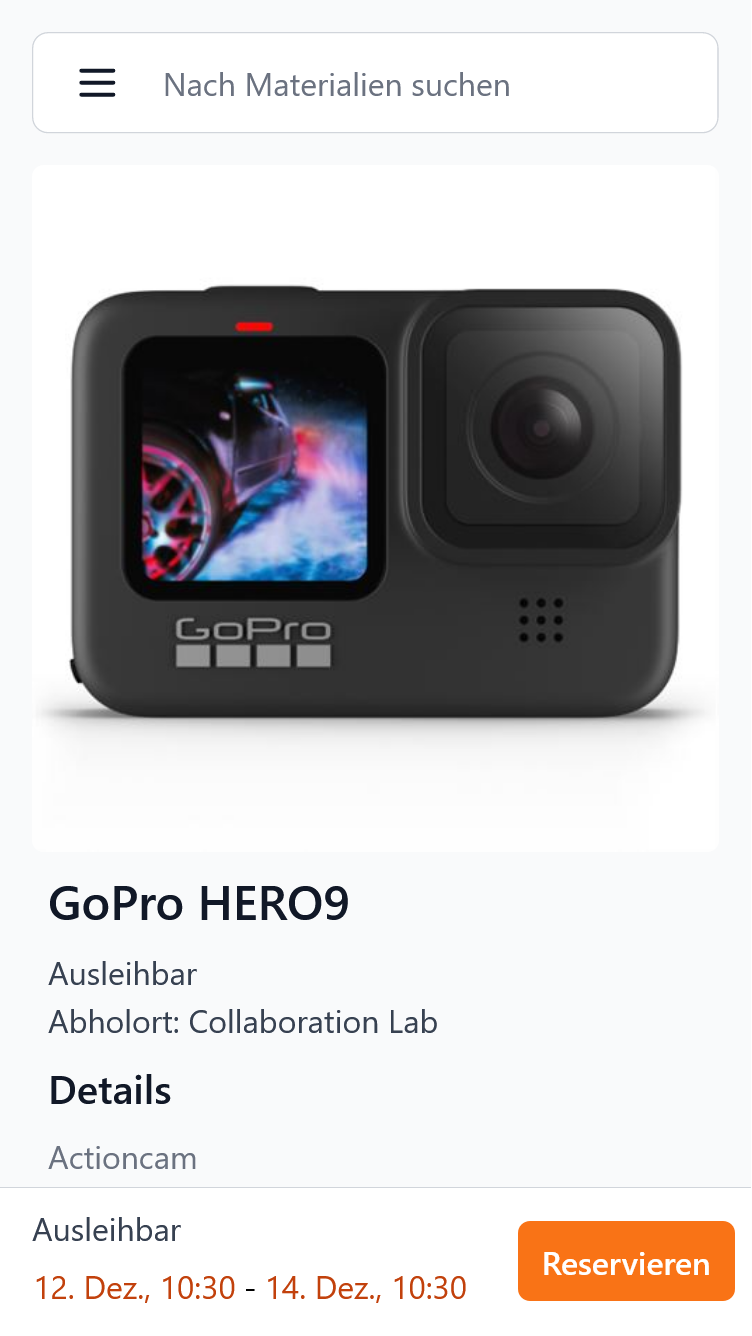
\includegraphics[scale=0.17]{Bilder/Dialgobeispiel/mit datum .png}\hspace{1em}
    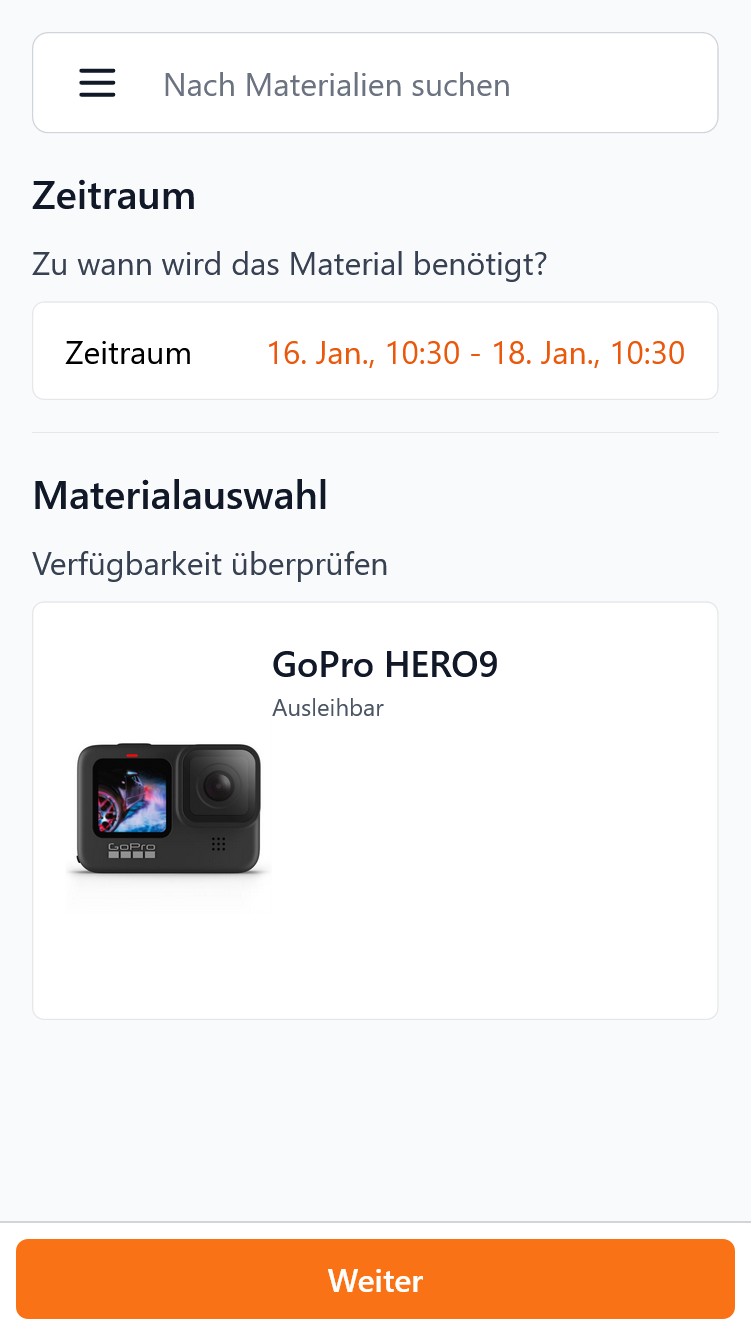
\includegraphics[scale=0.17]{Bilder/Dialgobeispiel/Falsche Uhrzeit.png}
    \caption{Dialogbeispiel 3: Kalender, Detailansicht mit Zeitangabe, Überblick}\label{fig:datum}
\end{figure}
\begin{figure}[p]
    \centering
    \includegraphics[scale=0.17]{Bilder/Dialgobeispiel/datumänderung.png}\hspace{1em}
    \includegraphics[scale=0.17]{Bilder/Dialgobeispiel/Bestätigung.png} \hspace{1em}
    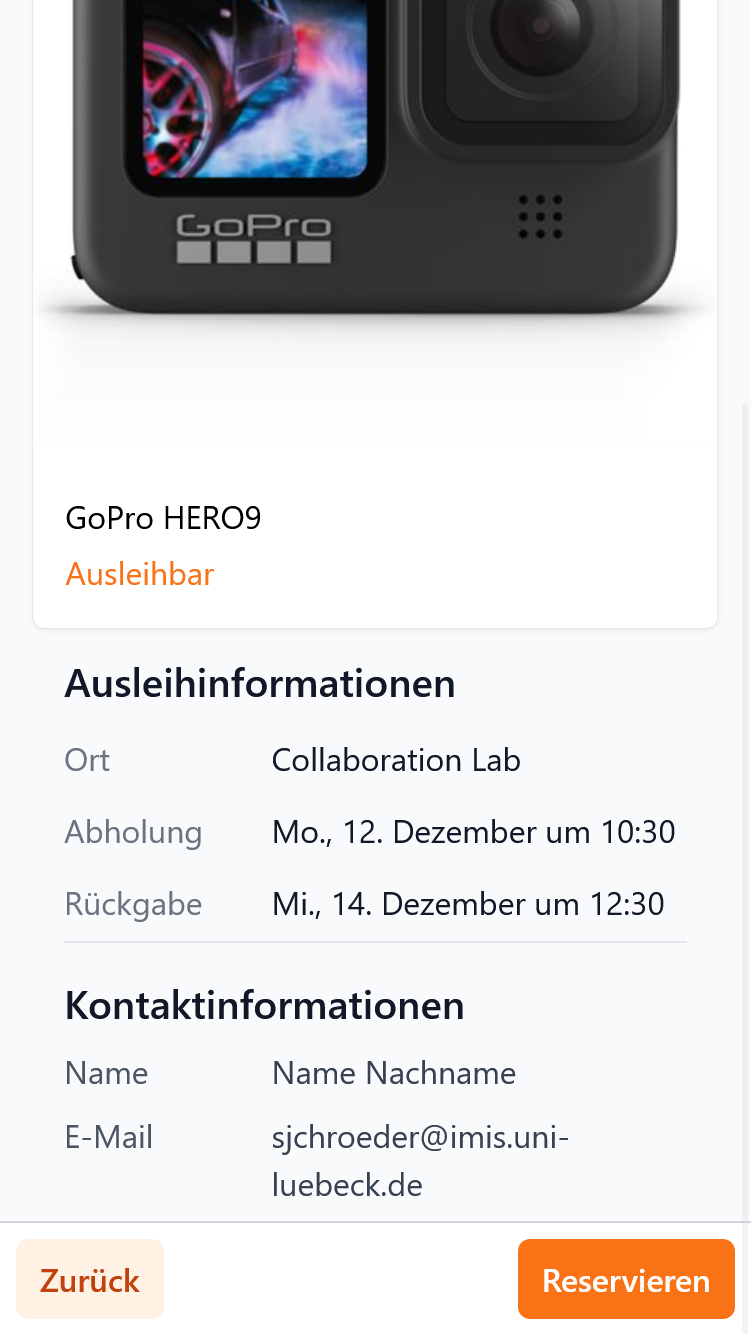
\includegraphics[scale=0.17]{Bilder/Dialgobeispiel/Zsuammenfassung.png}
    \caption{Dialogbeispiel 4: Kalender (Zeit ändern), Reservierungszusammenfassung}\label{fig:geandert}
\end{figure}

Da sich die Gruppe nicht sicher ist, welches Mikrofon für die Aufnahme eines
Voiceover sinnvoll ist, suchen sie zunächst in der Ausleih-App nach \enquote{Mikrofonen} und
sehen, dass Georg Fink für diese zuständig ist. Daraufhin verfasst Mila eine
E-Mail an Herrn Fink, in der sie um eine Mikrofon-Empfehlung für Voiceovers
bittet. Nachdem dieser mit zwei Vorschlägen geantwortet hat, sucht Mila nach
jenen unter der Angabe ihres Ausleihzeitraums. Direkt stellt Mila fest, dass
nur eines der Mikrofone in dem Ausleihzeitraum ausleihbar ist und reserviert
dieses.

Georg ist als \ac{wimi} am \ac{imis} für zwei Labore zuständig, in
denen Material ausgeliehen werden kann. Zum Feierabend überprüft er sein
Verwaltungsdashboard auf dem Desktop in der Ausleih-App. Er sieht, dass eine neue
Reservierung für Montag um 10:30 Uhr von Mila eingegangen ist (\ref{fig:georg}).

Da sich Mila am Sonntag nicht sicher ist, wo die Materialien abgeholt werden
sollen, schaut sie erneut in der Ausleih-App nach und findet den Abholort auf
der Dashboardansicht.

Nach der Vorlesung am Montag macht sich Mila auf den Weg in das Gebäude 64 zum
Abholort: Techniklabor. Georg wartet dort bereits auf Mila und erklärt ihr, was
sie bei der Nutzung der \textit{GoPro} beachten sollte. Nachdem Mila gegangen ist, trägt
Georg auf seinem Smartphone ein, dass die Materialien abgeholt wurden (\ref{fig:georg2}). Sobald
Georg die Abholung bestätigt hat, wird der Status in der internen Datenbank von
Snipe-IT geändert (\ref{fig:georg2}).

\begin{figure}[p]
    \centering
    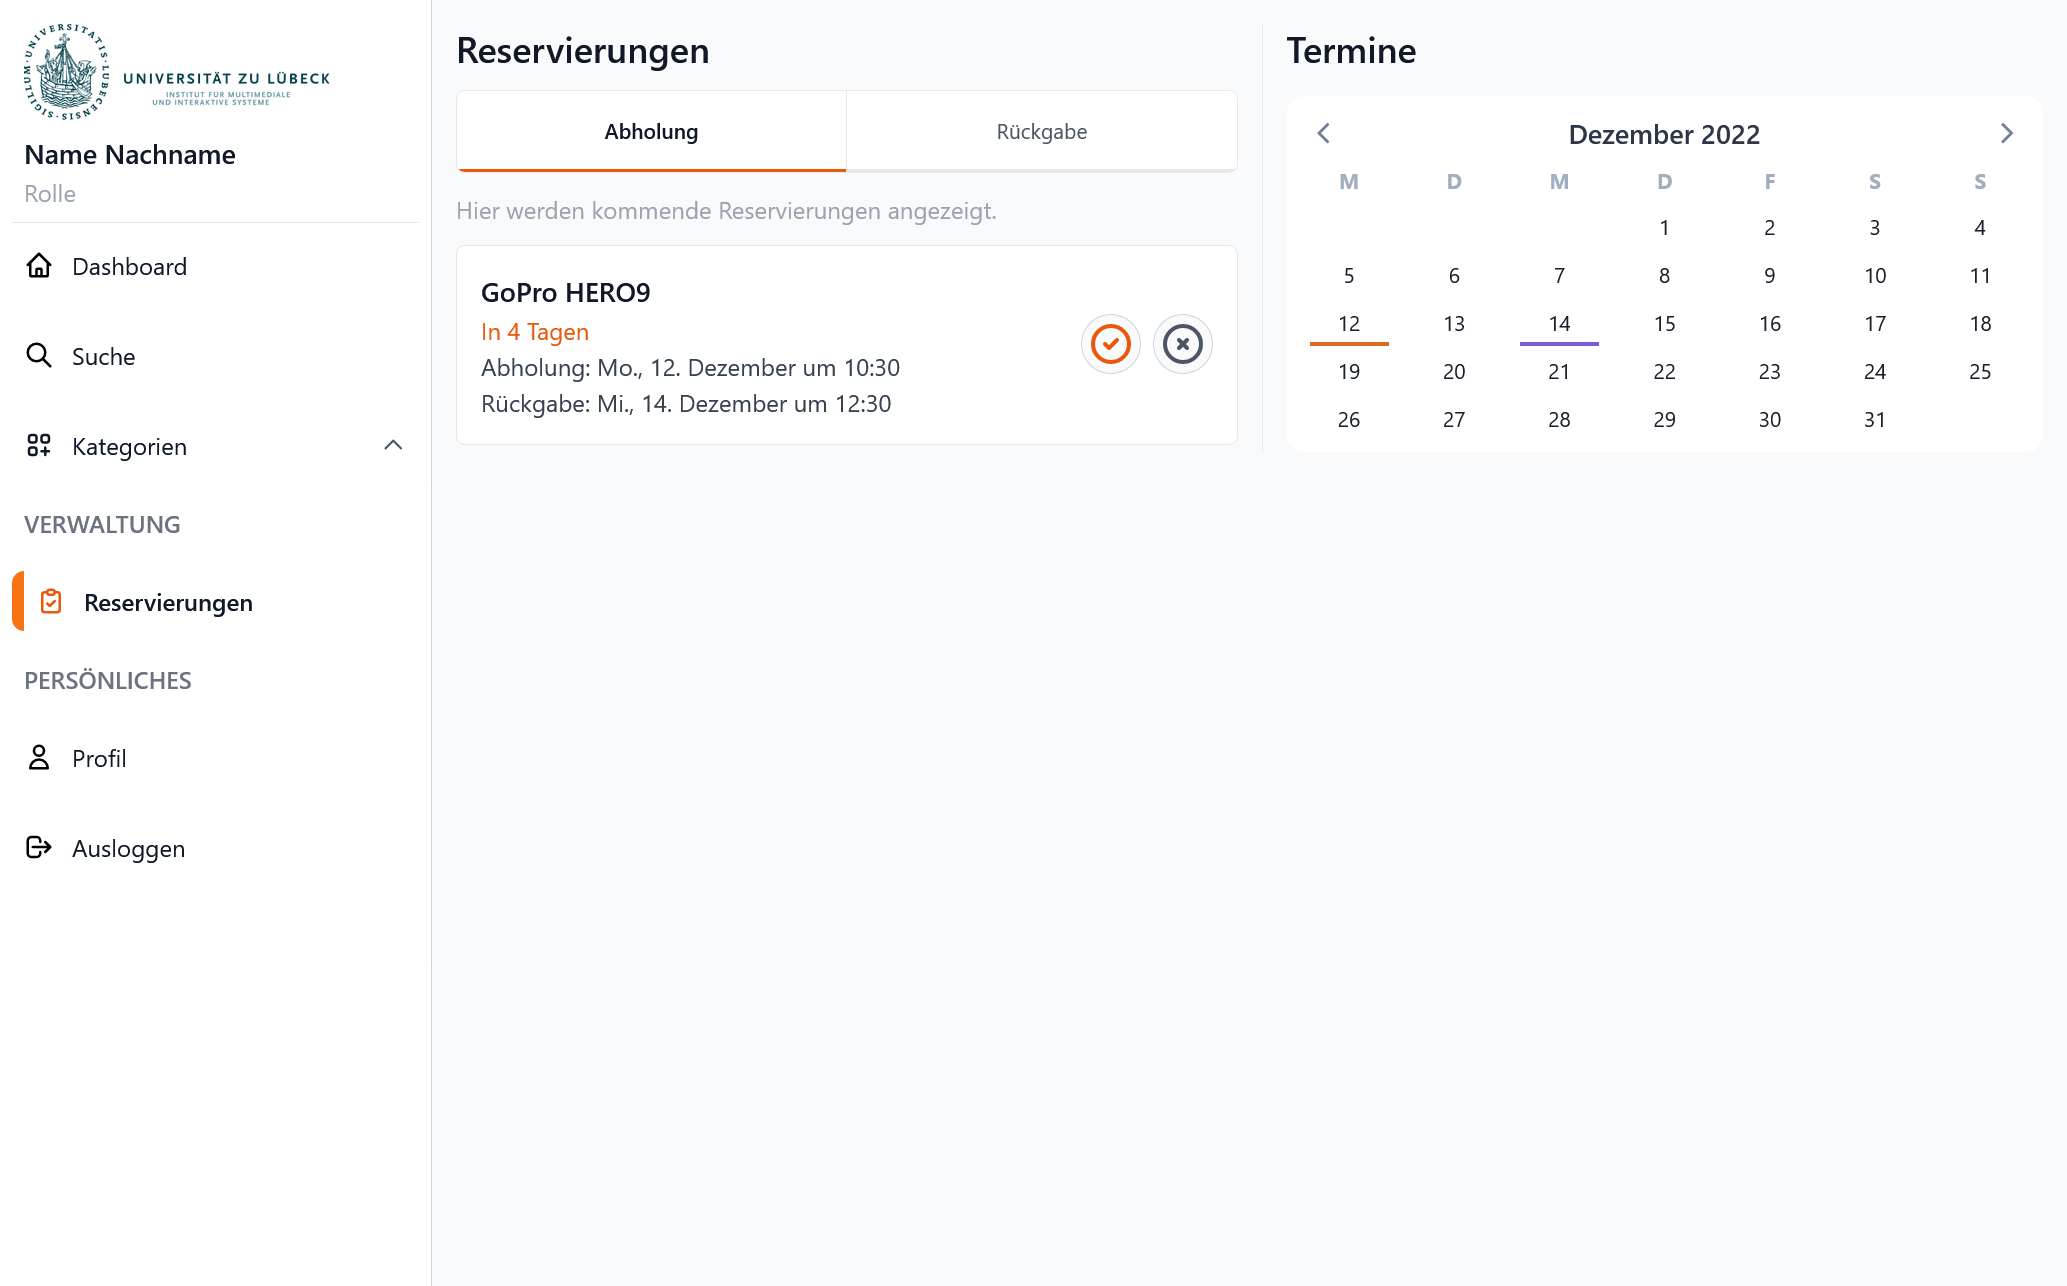
\includegraphics[scale=0.25]{Bilder/Dialgobeispiel/Verwaltung.png}
    \caption{Dialogbeispiel 5: Desktop - Verwaltung}\label{fig:georg}
\end{figure}
\begin{figure}[p]
    \centering
    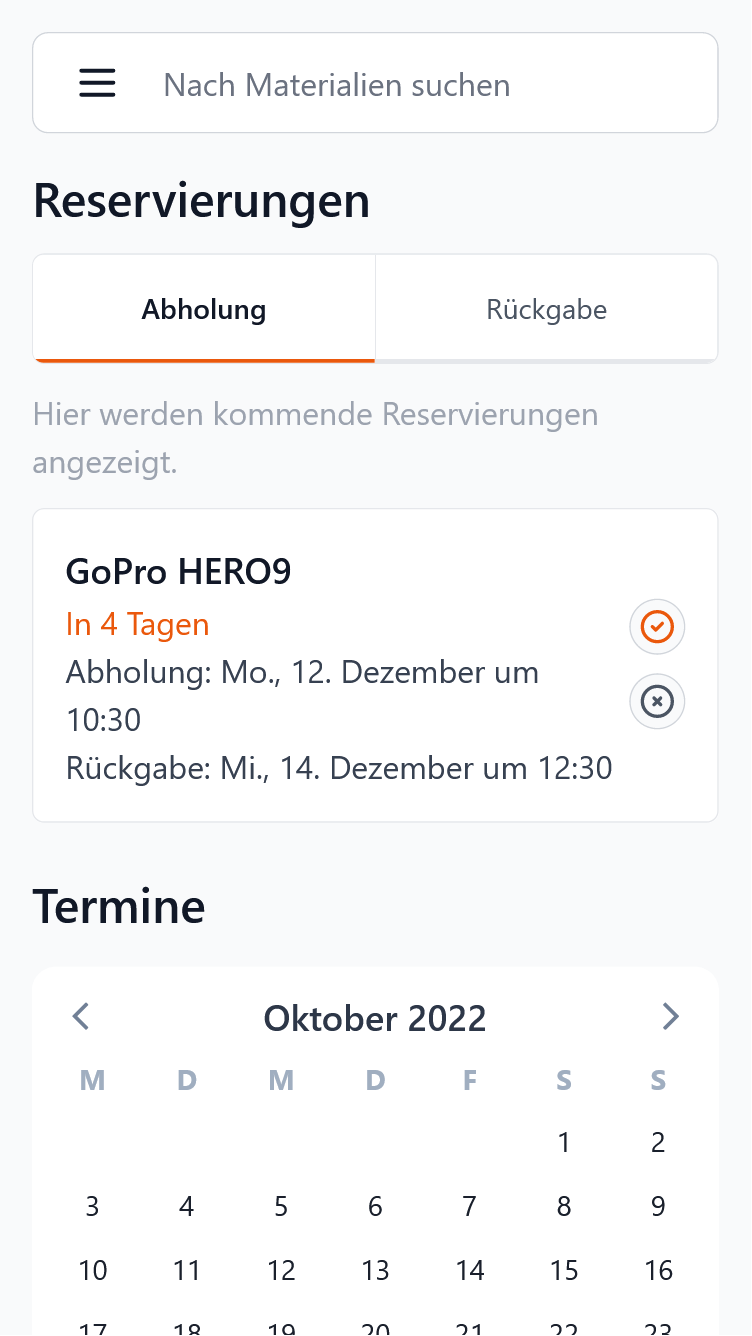
\includegraphics[scale=0.17]{Bilder/Dialgobeispiel/Reservierung Abholung.png}
    \caption{Dialogbeispiel 6: Mobile Ansicht - Verwaltung}
    \label{fig:georg2}
\end{figure}

\newpage
Laura Eggers ist ebenfalls \ac{wimi} am \ac{imis} und möchte für eine
Studie ein Mikrofon ausleihen. Da sie Zugriff auf Snipe-IT hat, schaut sie
zunächst dort nach dem gewünschten Material und stellt fest, dass dieses
\textit{herausgegeben} ist. Daraufhin ruft sie die URL
\textit{https://snipe-it-companion.de/} auf und reserviert das Mikrofon im
gewünschten Zeitraum. Am Abholtag entnimmt sie das Asset und bestätigt die
Abholung auf ihrem Smartphone. Nach der Bestätigung wird der Assetstatus in
Snipe-IT auf \enquote{herausgegeben} aktualisiert \ref{fig:georg5}. 
\begin{figure}[h]
    \centering
    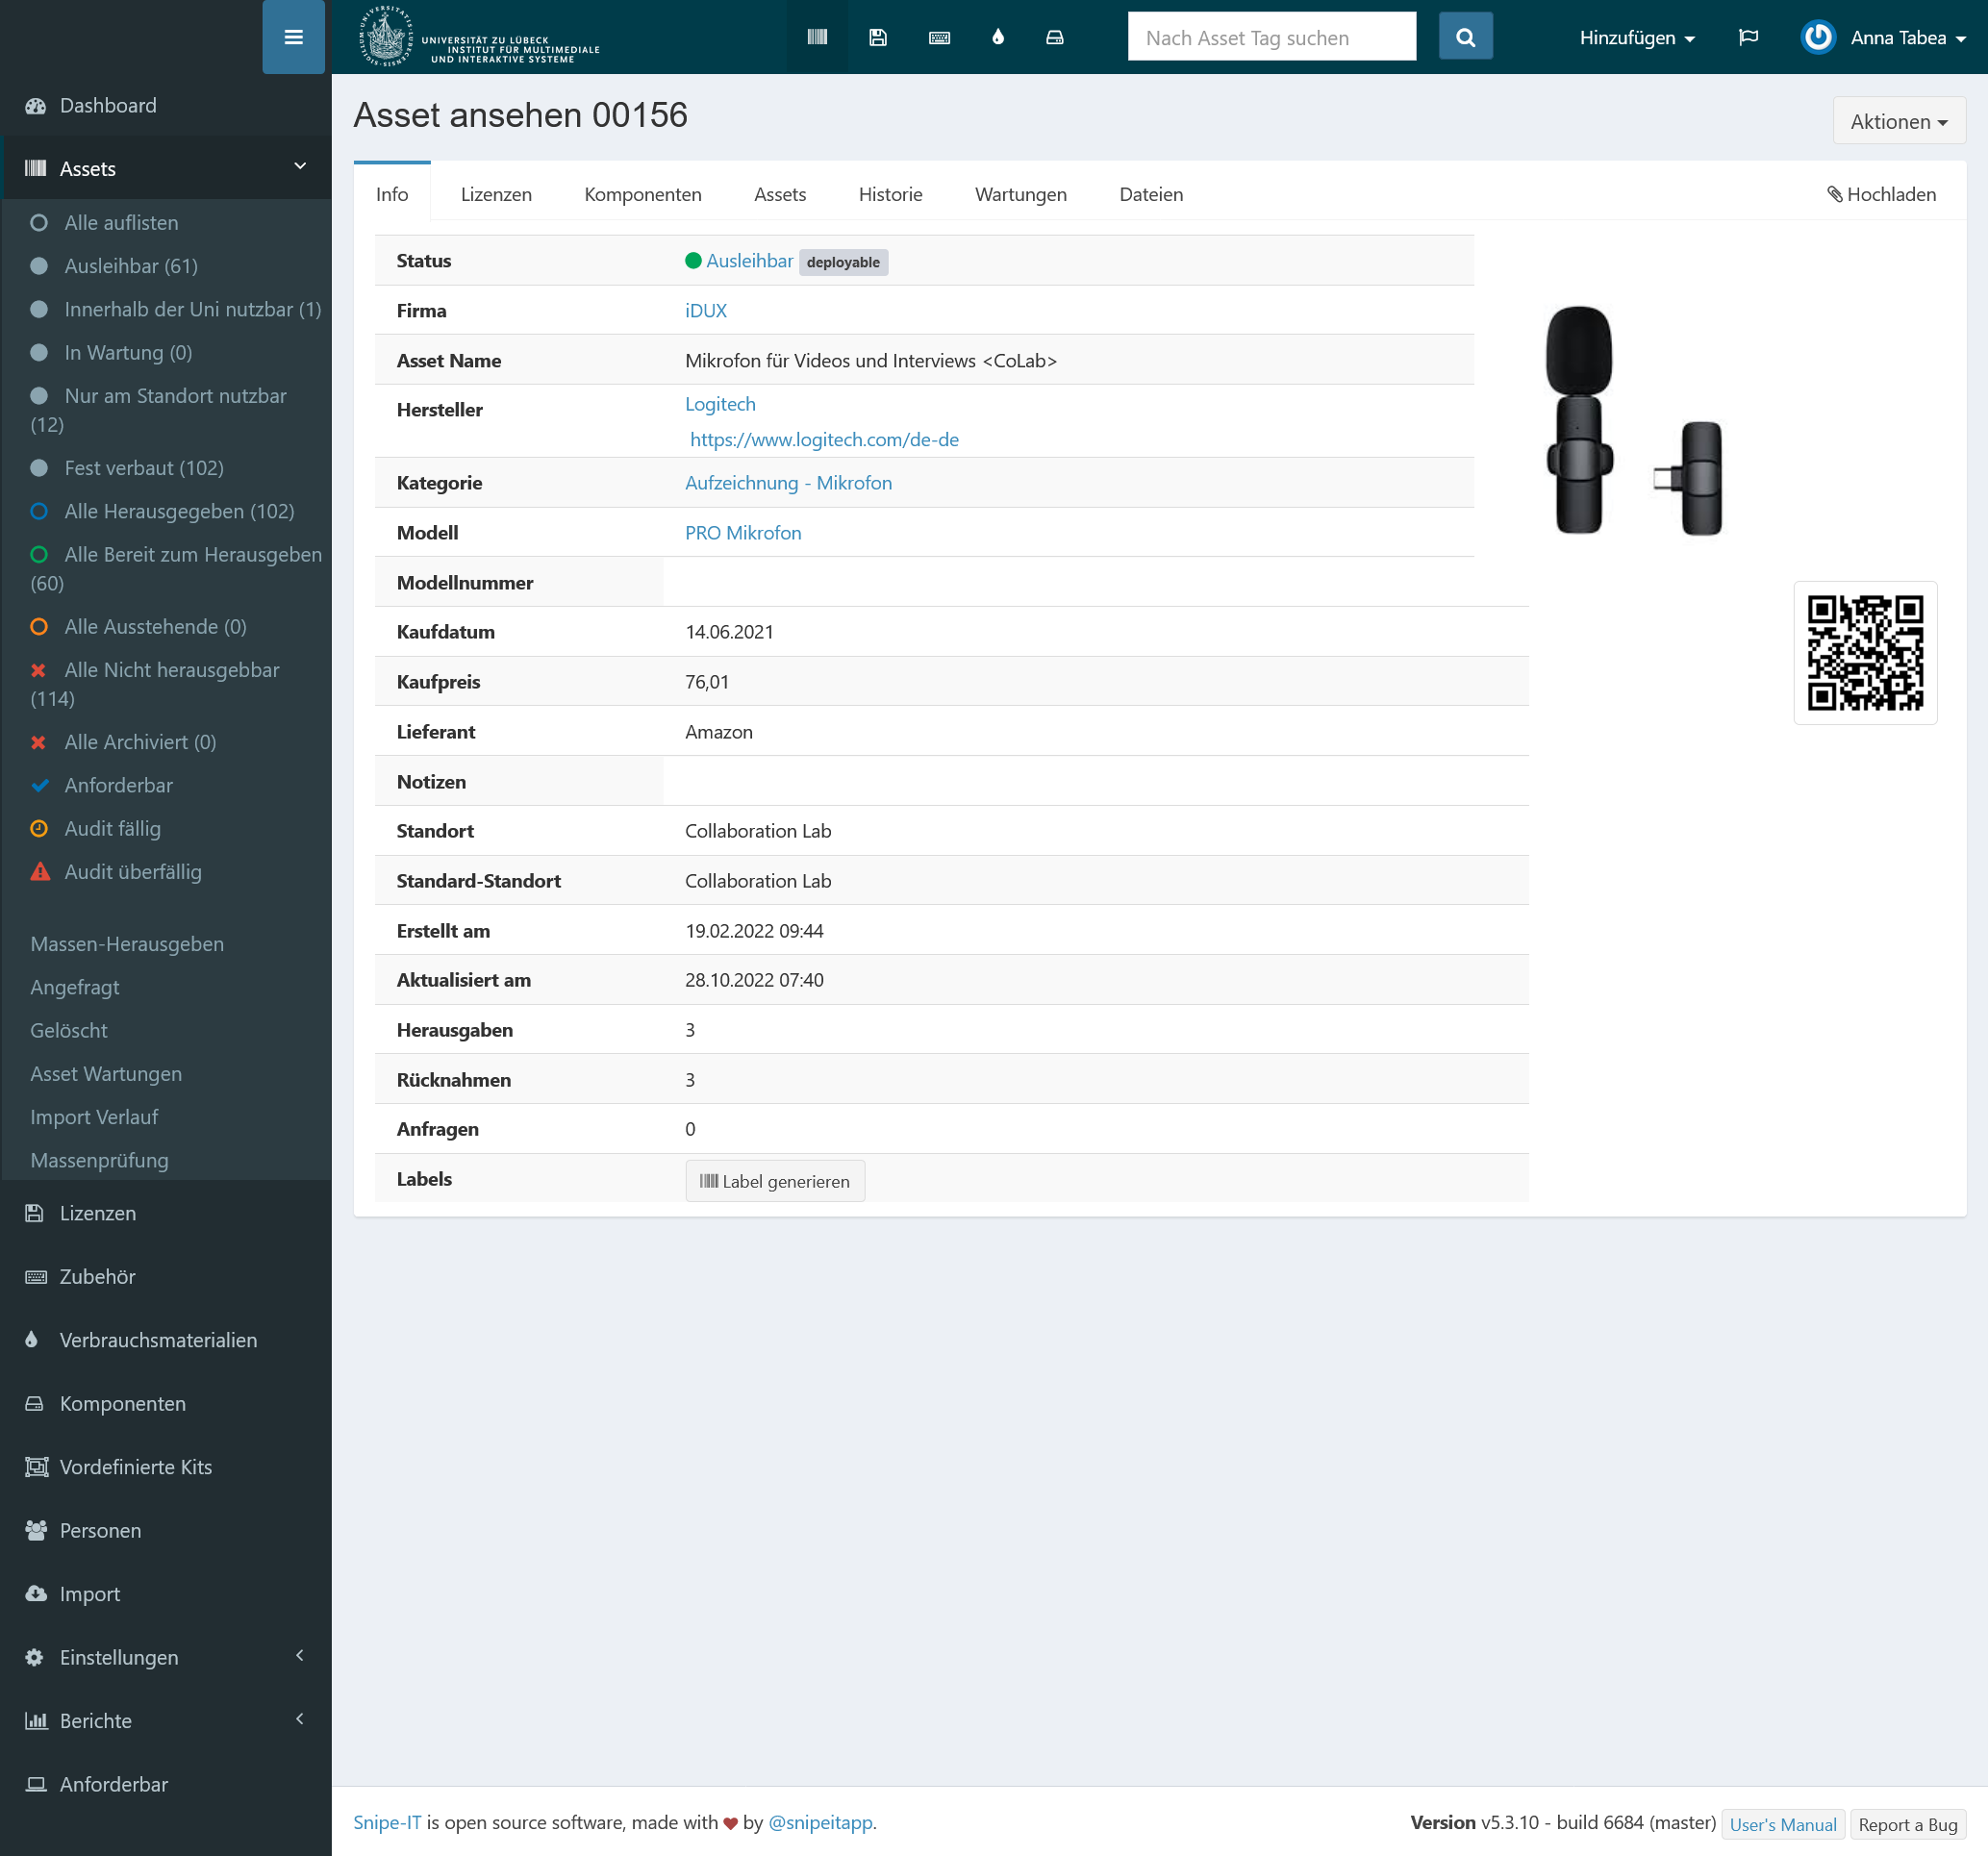
\includegraphics[scale=0.2]{Bilder/snipeit.png}
    \caption{Dialogbeispiel 7: Assetansicht in Snipe-IT}\label{fig:georg5}
\end{figure}

\newpage
Milas Gruppe stellt am Dienstag fest, dass ihnen der Ausleihzeitraum nicht
ausreicht und möchte diesen daher um einen Tag verlängern. Dafür öffnet sie die
Ausleih-App und sieht auf dem Dashboard unter dem Tab \textit{Laufende} ihre
Reservierungen. Daraufhin ändert sie die Daten der beiden Materialien auf
Donnerstag um 9:00 Uhr (\ref{fig:andern}). Georg wird die Verlängerung ebenfalls
in der Verwaltungsansicht angezeigt.
\begin{figure}[h]
    \centering
    \includegraphics[scale=0.17]{Bilder/Dialgobeispiel/laufende nach änderung.png}\hspace{1em}
    \includegraphics[scale=0.17]{Bilder/Dialgobeispiel/Datum ändern 2.png}\hspace{1em}
    \caption{Dialogbeispiel 8: Dashboard, Zeitraum verlängern}\label{fig:andern}
\end{figure}

Am Donnerstag um 9:00 Uhr wartet Mila bereits auf Georg, welcher die
Materialien entgegennimmt und in seinem Büro die Rückgabe bestätigt (\ref{fig:zuruck}).

Im vierten Semester möchte Mila das Mikrofon für das Modul \textit{\ac{ide}}
ausleihen, um wieder ein Voiceover aufnehmen zu können. Sie findet das Mikrofon
unter \textit{zurückgegeben} und leiht das Material erneut aus (\ref{fig:zuruck}).
\begin{figure}[h]
    \centering
    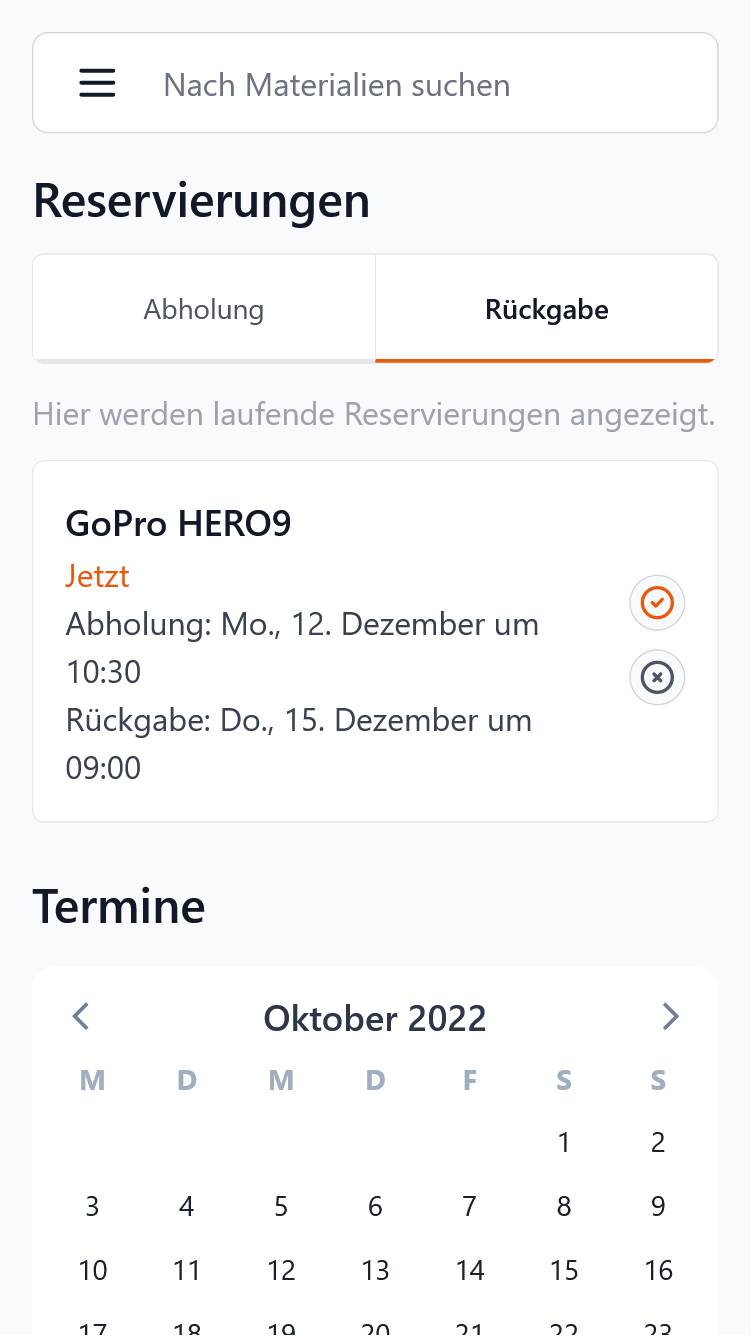
\includegraphics[scale=0.17]{Bilder/Dialgobeispiel/Altes Datum.png}\hspace{1em}
    \includegraphics[scale=0.17]{Bilder/Dialgobeispiel/Zurück.png}\hspace{1em}
    \caption{Dialogbeispiel 9: Verwaltungsrückgabe und Dashboardrückgabe}\label{fig:zuruck}
\end{figure}